\chapter{APPLICATION NUMÉRIQUE}
\thispagestyle{empty}

\section{Analyse des coûts}

Cette section présente une analyse détaillée des coûts du projet, considérant toutes les ressources qui contribuent à la réalisation du système. Suivant les directives, les ressources économiques et les ressources informatiques sont prises en compte.

\subsection{Ressources informatiques}

Les ressources informatiques primaires sont résumées dans le Tableau~\ref{tab:compute-resources}.

\begin{table}[htbp]
\centering
\caption{Ressources informatiques utilisées dans le projet.}
\label{tab:compute-resources}
\begin{tabular}{llr}
\toprule
\textbf{Ressource} & \textbf{Spécification} & \textbf{Quantité} \\
\midrule
GPU & NVIDIA RTX 4070 Laptop (8Go VRAM) & 1 \\
CPU & AMD Ryzen 9 8945HS (4GHz) & 1 \\
RAM & DDR5 32Go & 32 Go \\
Stockage & NVMe SSD & 512 Go \\
\bottomrule
\end{tabular}
\end{table}

\subsection{Taille des données}

Les tailles des données pour la collection Custom-WikiCS sont présentées dans le Tableau~\ref{tab:dataset-sizes}.

\begin{table}[htbp]
\centering
\caption{Exigences de stockage des données.}
\label{tab:dataset-sizes}
\begin{tabular}{lr}
\toprule
\textbf{Composant} & \textbf{Taille} \\
\midrule
Données brutes WikiCS (format PyG) & 202.2 Mo \\
Embeddings BGE-M3 (11\,367 $\times$ 1024 $\times$ float32) & 21.3 Mo \\
Embeddings Node2Vec (11\,367 $\times$ 128 $\times$ float32) & 6.5 Mo \\
Cache d'embeddings combiné & 27.8 Mo \\
Matrice d'adjacence (creuse) & 8.2 Mo \\
\textbf{Total} & \multicolumn{1}{r}{238.2 Mo} \\
\bottomrule
\end{tabular}
\end{table}

Les données brutes du graphe WikiCS dominent l'empreinte de stockage à 202.2 Mo, tandis que le cache d'embeddings combiné ne représente que 27.8 Mo (~12\% du total). Le pré-calcul des embeddings hors ligne économise un temps de recalcul significatif.

\subsection{Utilisation mémoire GPU}

Les exigences de mémoire GPU varient selon le modèle et la configuration, comme montré dans le Tableau~\ref{tab:gpu-memory}.

\begin{table}[htbp]
\centering
\caption{Utilisation mémoire GPU par configuration de modèle.}
\label{tab:gpu-memory}
\begin{tabular}{lrr}
\toprule
\textbf{Modèle} & \textbf{Configuration} & \textbf{Mémoire GPU} \\
\midrule
GCN & 2 couches, 128 unités cachées & 2--3 Go \\
GAT & 2 couches, 8 têtes, 128 unités cachées & 4--6 Go \\
Inférence BGE-M3 (batch) & 11\,367 nœuds & 3--4 Go \\
Combiné (entraînement) & GAT + embeddings sur GPU & 6--8 Go \\
\bottomrule
\end{tabular}
\end{table}

Les 8Go de VRAM du RTX 4070 sont suffisants pour toutes les expériences actuelles mais laissent une marge limitée pour des tailles de lot plus grandes ou des modèles plus complexes.

\subsection{Temps d'entraînement}

Le Tableau~\ref{tab:training-time} présente les estimations de temps d'entraînement pour différentes configurations sur l'ordinateur portable RTX 4070.

\begin{table}[htbp]
\centering
\caption{Estimations de temps d'entraînement pour 100 époques.}
\label{tab:training-time}
\begin{tabular}{lrr}
\toprule
\textbf{Modèle} & \textbf{Temps par Époque} & \textbf{Total (100 époques)} \\
\midrule
GCN (base) & 8--12 sec & 13--20 min \\
GAT (2 couches, 4 têtes) & 15--25 sec & 25--40 min \\
GAT (3 couches, 8 têtes) & 30--45 sec & 50--75 min \\
\bottomrule
\end{tabular}
\end{table}

L'expérience de base GCN (100 époques) se termine en environ 15--20 minutes sur le matériel disponible.

\subsection{Temps de génération des embeddings}

Le Tableau~\ref{tab:embedding-time} présente le temps requis pour générer les embeddings de phrases.

\begin{table}[htbp]
\centering
\caption{Temps de génération des embeddings.}
\label{tab:embedding-time}
\begin{tabular}{lrr}
\toprule
\textbf{Modèle} & \textbf{Temps (11\,367 articles)} & \textbf{Matériel} \\
\midrule
BAAI/bge-m3 (1024-dim) & 30--60 min & GPU RTX 4070 \\
mGTE-modernbert (768-dim) & 20--40 min & GPU RTX 4070 \\
SVD-Node2Vec (128-dim) & 2--5 min & CPU \\
\bottomrule
\end{tabular}
\end{table}

La génération d'embeddings BGE-M3 est un coût unique; les embeddings sont mis en cache pour les expériences subséquentes.

\subsection{Consommation d'énergie}

Le Tableau~\ref{tab:power-consumption} présente les estimations de consommation électrique.

\begin{table}[htbp]
\centering
\caption{Consommation électrique par session d'entraînement.}
\label{tab:power-consumption}
\begin{tabular}{lrr}
\toprule
\textbf{Composant} & \textbf{Consommation} & \textbf{Durée (entraînement GCN)} \\
\midrule
GPU (RTX 4070 Laptop) & 140W (pic) / 100W (moy) & 15--20 min \\
Système (CPU, RAM, SSD) & 60W & 15--20 min \\
Total & 160--200W (moy ~160W) & 15--20 min \\
\midrule
\textbf{Énergie par Exécution} & \multicolumn{2}{c}{0.06--0.10 kWh} \\
\bottomrule
\end{tabular}
\end{table}

En supposant 20 exécutions d'entraînement complètes (exploration d'hyperparamètres, études d'ablation), la consommation d'énergie totale pour l'entraînement GNN est d'environ 1.2--2.0 kWh.

\subsection{Ressources humaines}

Le Tableau~\ref{tab:human-resources} présente l'effort humain estimé pour le projet.

\begin{table}[htbp]
\centering
\caption{Estimations de l'effort humain (heures).}
\label{tab:human-resources}
\begin{tabular}{lr}
\toprule
\textbf{Activité} & \textbf{Heures} \\
\midrule
Enquête littéraire & 60 heures \\
Construction du dataset (Custom-WikiCS) & 40 heures \\
Génération et mise en cache des embeddings & 10 heures \\
Analyse graphique (Report-4) & 30 heures \\
Implémentation et entraînement du modèle GNN & 50 heures \\
Développement du système de recommandation (Report-5) & 40 heures \\
Rédaction de rapports (tous mid-reports + final) & 80 heures \\
\midrule
\textbf{Total} & \textbf{310 heures} \\
\bottomrule
\end{tabular}
\end{table}

\section{Premiers résultats}

Cette section présente les résultats expérimentaux initiaux obtenus à ce jour.

\subsection{Analyse structurelle du graphe}

Avant le développement du modèle, une analyse structurelle complète du graphe Custom-WikiCS a été réalisée (Report-4). Les principales conclusions sont résumées ci-dessous.

\begin{figure}[H]
    \centering
    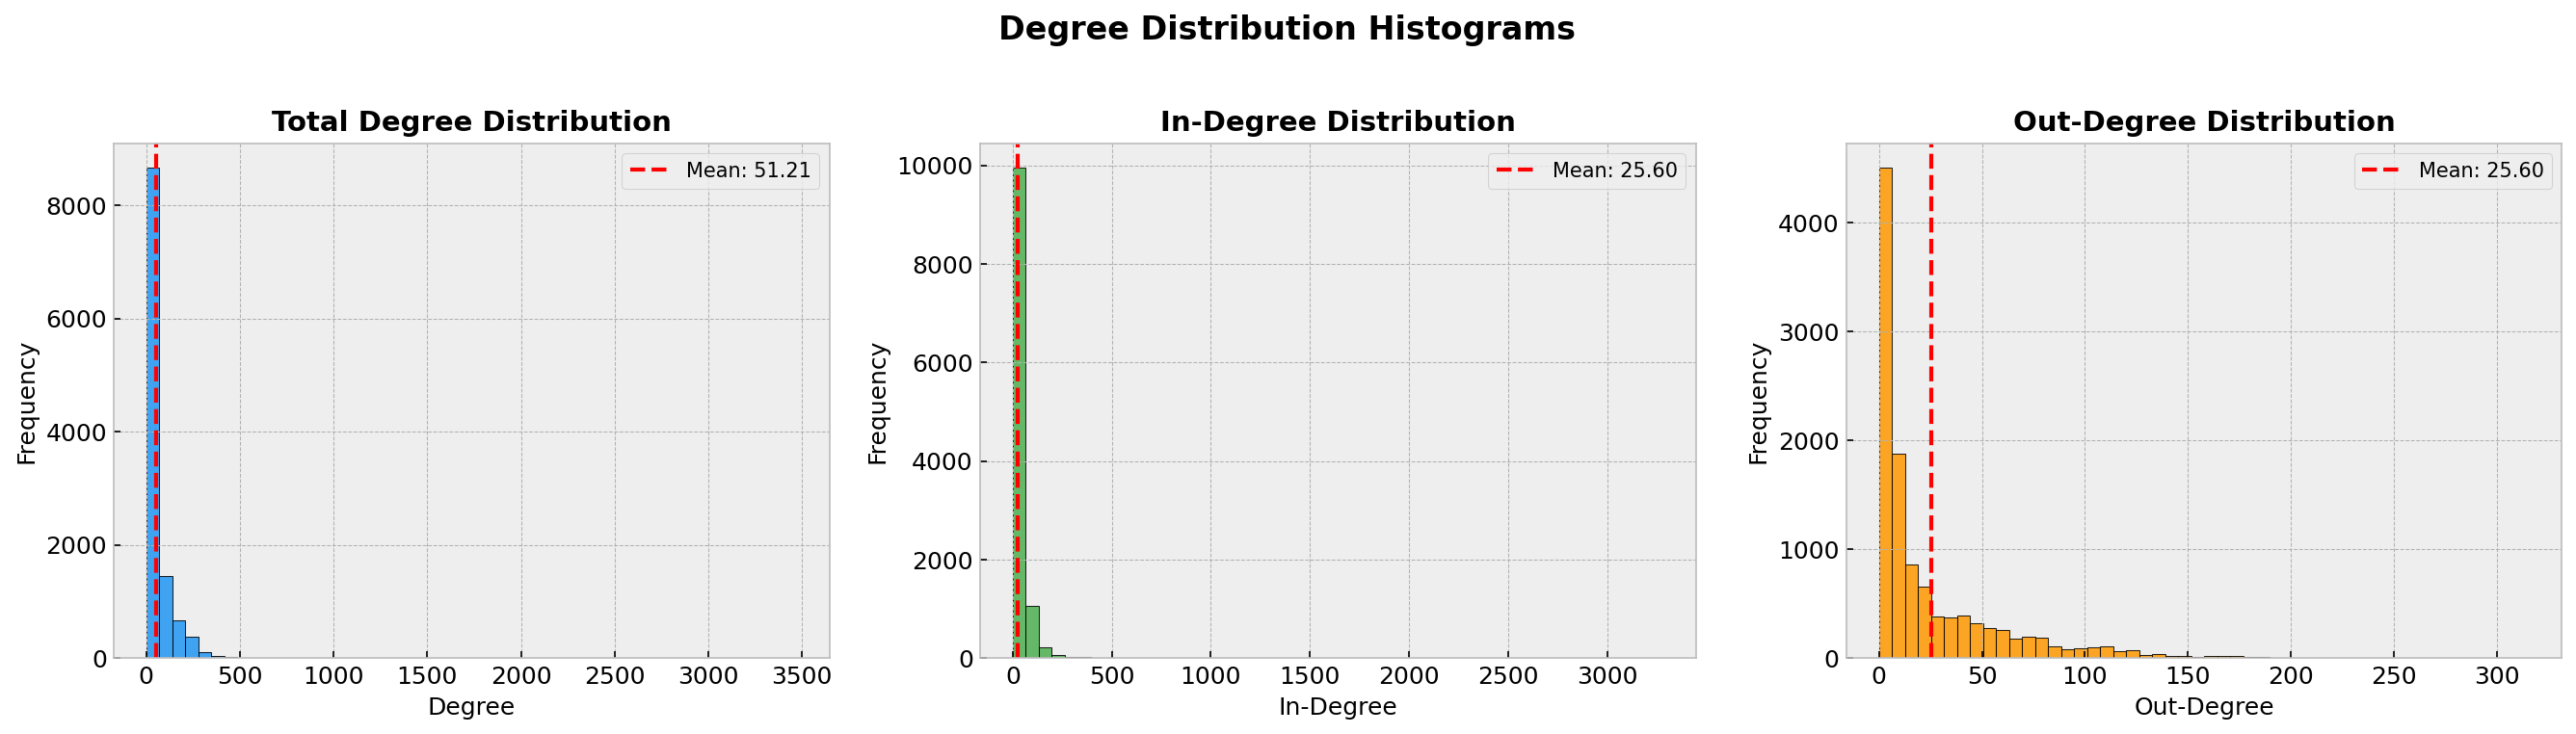
\includegraphics[width=0.75\textwidth]{figures/degree-distribution.png}
    \caption{Distribution des degrés du graphe Custom-WikiCS nettoyé.}
    \label{fig:degree-dist}
\end{figure}

La distribution des degrés (Figure~\ref{fig:degree-dist}) suit un patron de loi de puissance, caractéristique des réseaux sans échelle. Le Tableau~\ref{tab:degree-stats} présente les statistiques des degrés.

\begin{table}[htbp]
\centering
\caption{Statistiques des degrés pour le graphe nettoyé.}
\label{tab:degree-stats}
\begin{tabular}{lrrrr}
\toprule
 & \textbf{Min} & \textbf{Max} & \textbf{Moyenne} & \textbf{Médiane} \\
\midrule
Degré Total & 1 & 3\,474 & 51.21 & 16 \\
Degré Entrant & 0 & 3\,283 & 25.60 & 4 \\
Degré Sortant & 0 & 316 & 25.60 & 10 \\
\bottomrule
\end{tabular}
\end{table}

\begin{figure}[H]
    \centering
    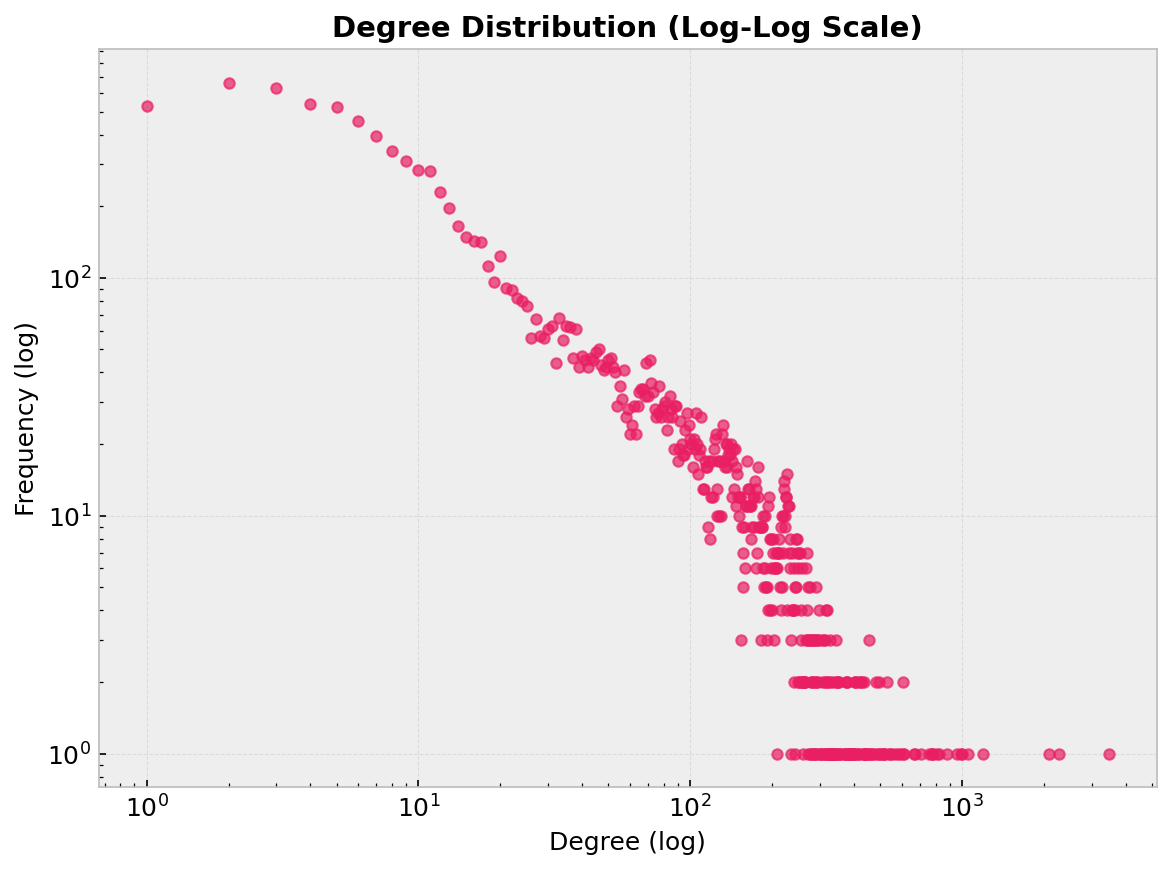
\includegraphics[width=0.65\textwidth]{figures/degree-log-log.png}
    \caption{Distribution des degrés en échelle log-log (évaluation loi de puissance).}
    \label{fig:degree-loglog}
\end{figure}

La relation approximativement linéaire sur les axes log-log (Figure~\ref{fig:degree-loglog}) confirme le comportement en loi de puissance, avec l'exposant ajusté $\alpha \approx 3.0$.

\begin{figure}[H]
    \centering
    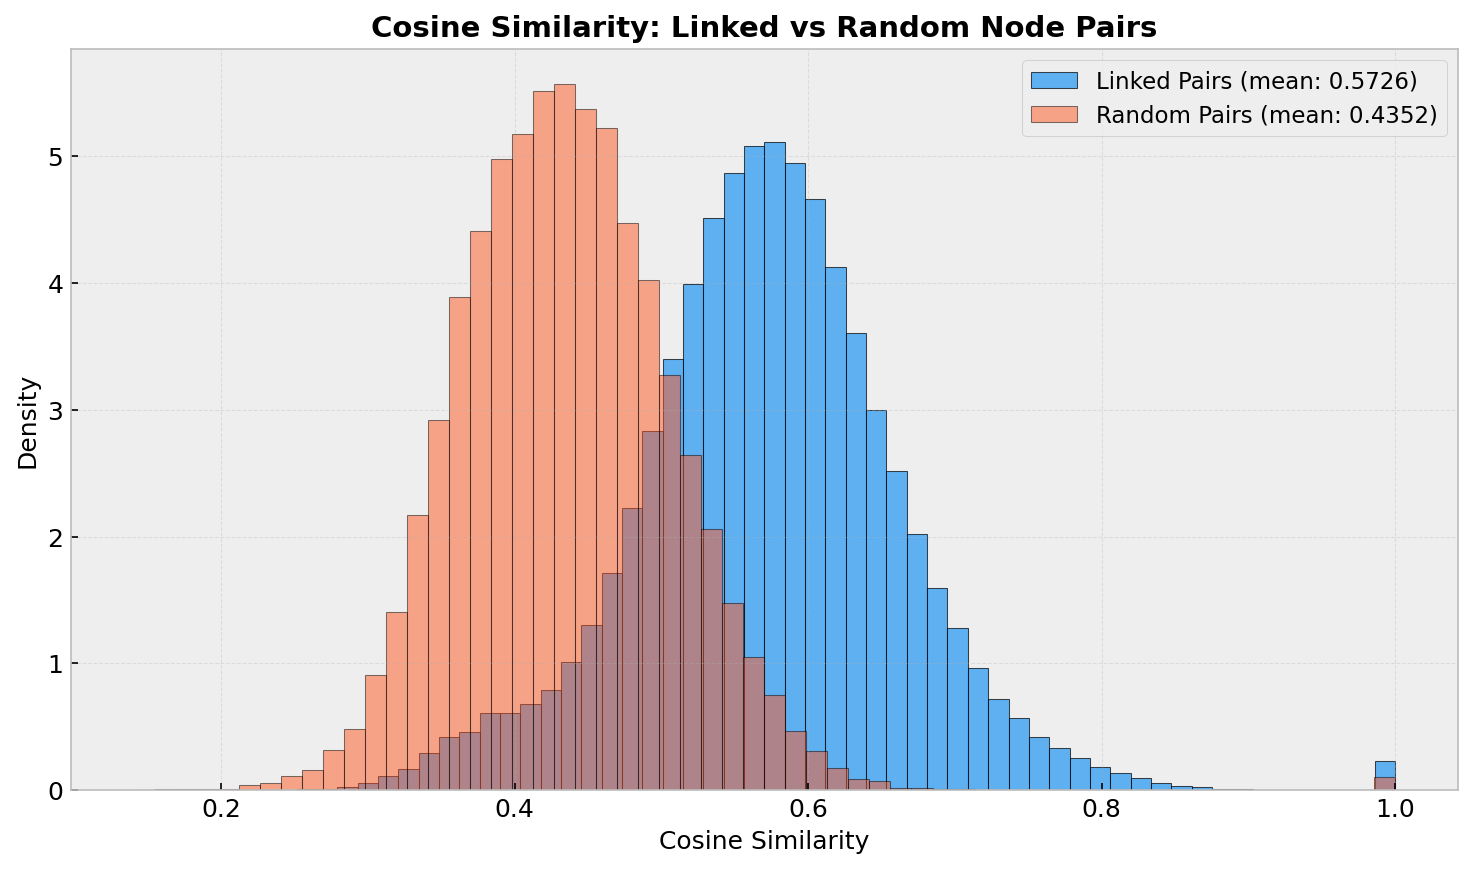
\includegraphics[width=0.75\textwidth]{figures/cosine-similarity-assortativity.png}
    \caption{Distribution de similarité cosinus: paires liées vs. paires aléatoires.}
    \label{fig:cosine-assort}
\end{figure}

Une découverte importante est que les paires d'articles liées présentent une similarité cosinus plus élevée (moyenne: 0.5726) que les paires aléatoires (moyenne: 0.4352), comme montré dans la Figure~\ref{fig:cosine-assort}. Cela confirme que les hyperliens encodent des relations sémantiques entre articles.

Les Figures~\ref{fig:pearson-assort} et~\ref{fig:euclidean-assort} présentent la même analyse en utilisant la corrélation de Pearson et la distance euclidienne, confirmant la découverte à travers les trois métriques.

\begin{figure}[H]
    \centering
    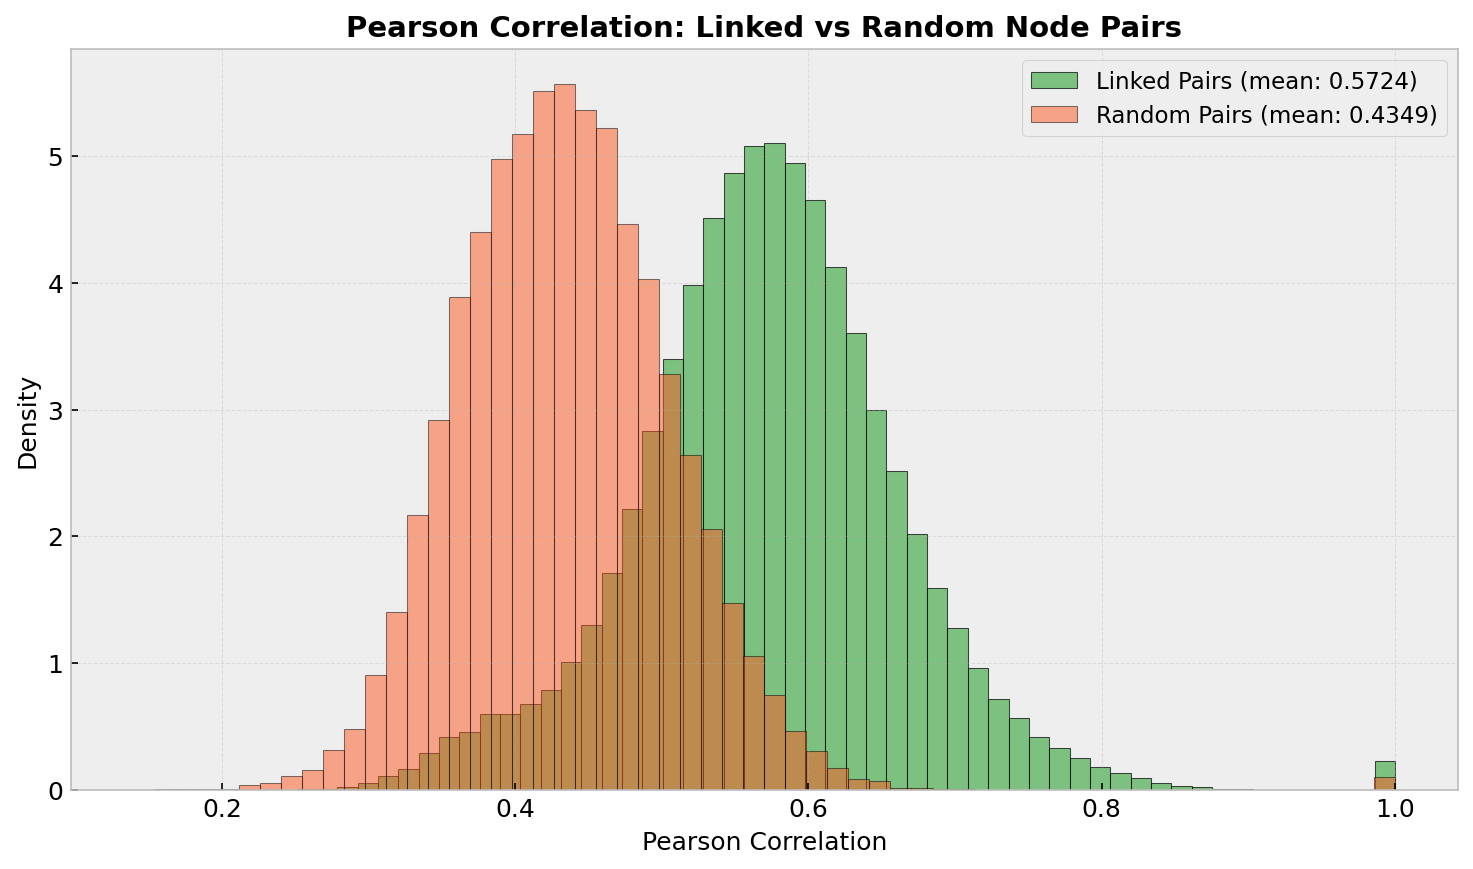
\includegraphics[width=0.75\textwidth]{figures/pearson-correlation-assortativity.png}
    \caption{Distribution de corrélation Pearson: paires liées vs. paires aléatoires.}
    \label{fig:pearson-assort}
\end{figure}

\begin{figure}[H]
    \centering
    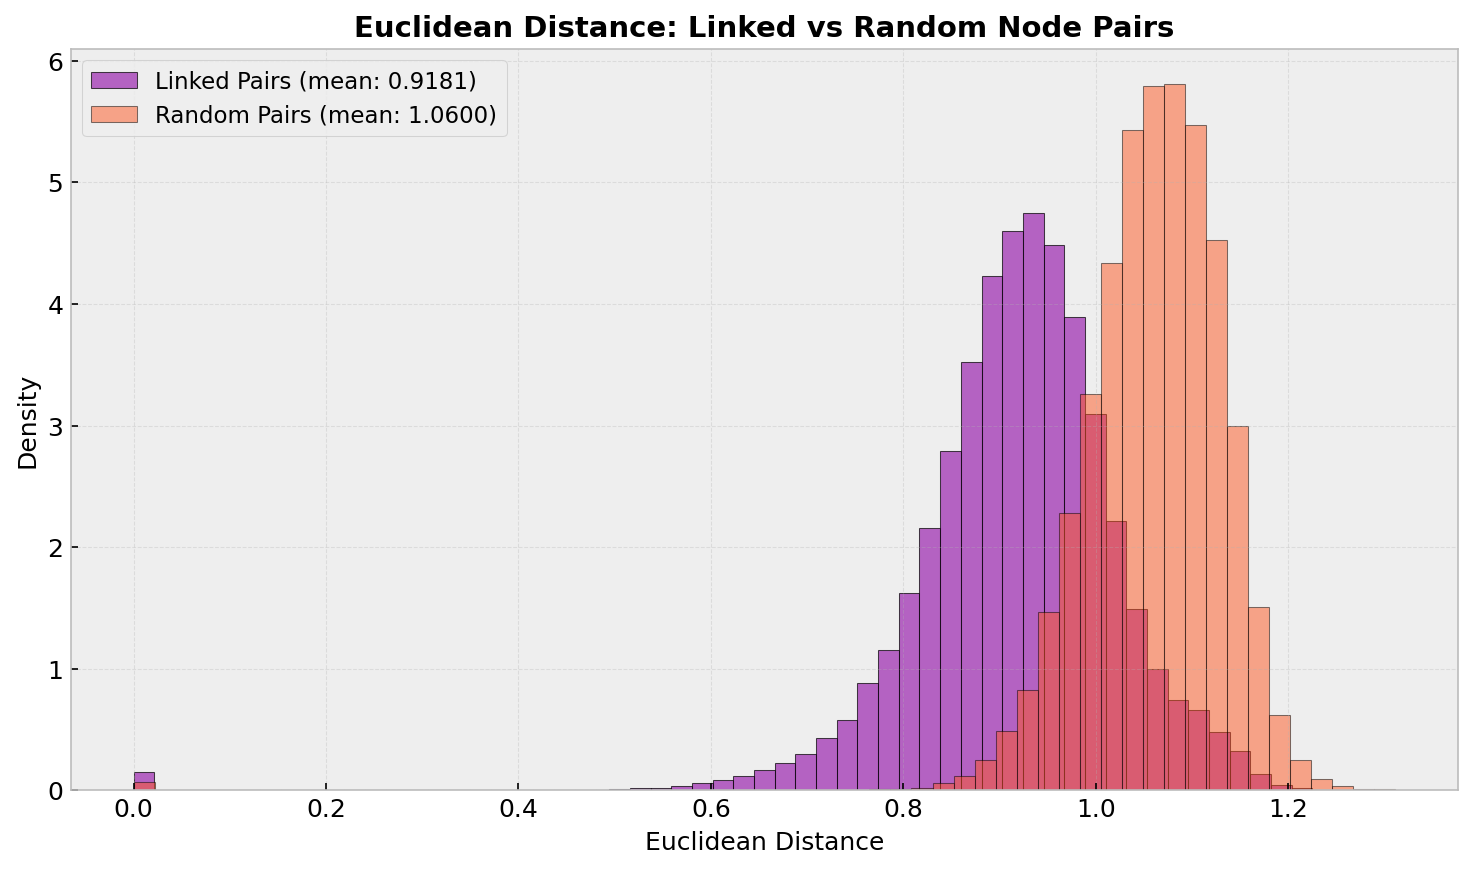
\includegraphics[width=0.75\textwidth]{figures/euclidean-distance-assortativity.png}
    \caption{Distribution de distance euclidienne: paires liées vs. paires aléatoires.}
    \label{fig:euclidean-assort}
\end{figure}

Le Tableau~\ref{tab:topic-link} résume les résultats d'assortativité thème-lien à travers les trois métriques.

\begin{table}[htbp]
\centering
\caption{Résumé de l'assortativité thème-lien pour toutes les trois métriques d'embedding.}
\label{tab:topic-link}
\begin{tabular}{lccccc}
\toprule
\textbf{Métrique} & \textbf{Liée Moy.} & \textbf{Liée É.-T.} & \textbf{Aléatoire Moy.} & \textbf{Aléatoire É.-T.} & \textbf{Diff} \\
\midrule
Similarité Cosinus   & 0.5726 & 0.0901 & 0.4352 & 0.0724 & $+0.1374$ \\
Corrélation Pearson & 0.5724 & 0.0902 & 0.4349 & 0.0725 & $+0.1375$ \\
Distance Euclidienne  & 0.9181 & 0.1089 & 1.0600 & 0.0773 & $-0.1419$ \\
\bottomrule
\end{tabular}
\end{table}

\subsection{Résultats de détection de communautés}

La détection de communautés par les algorithmes Louvain et Infomap révèle des amas topiques cohérents significatifs dans le graphe (Figures~\ref{fig:louvain-communities} et \ref{fig:infomap-communities}, et Tableau~\ref{tab:community-results}).

\begin{figure}[H]
    \centering
    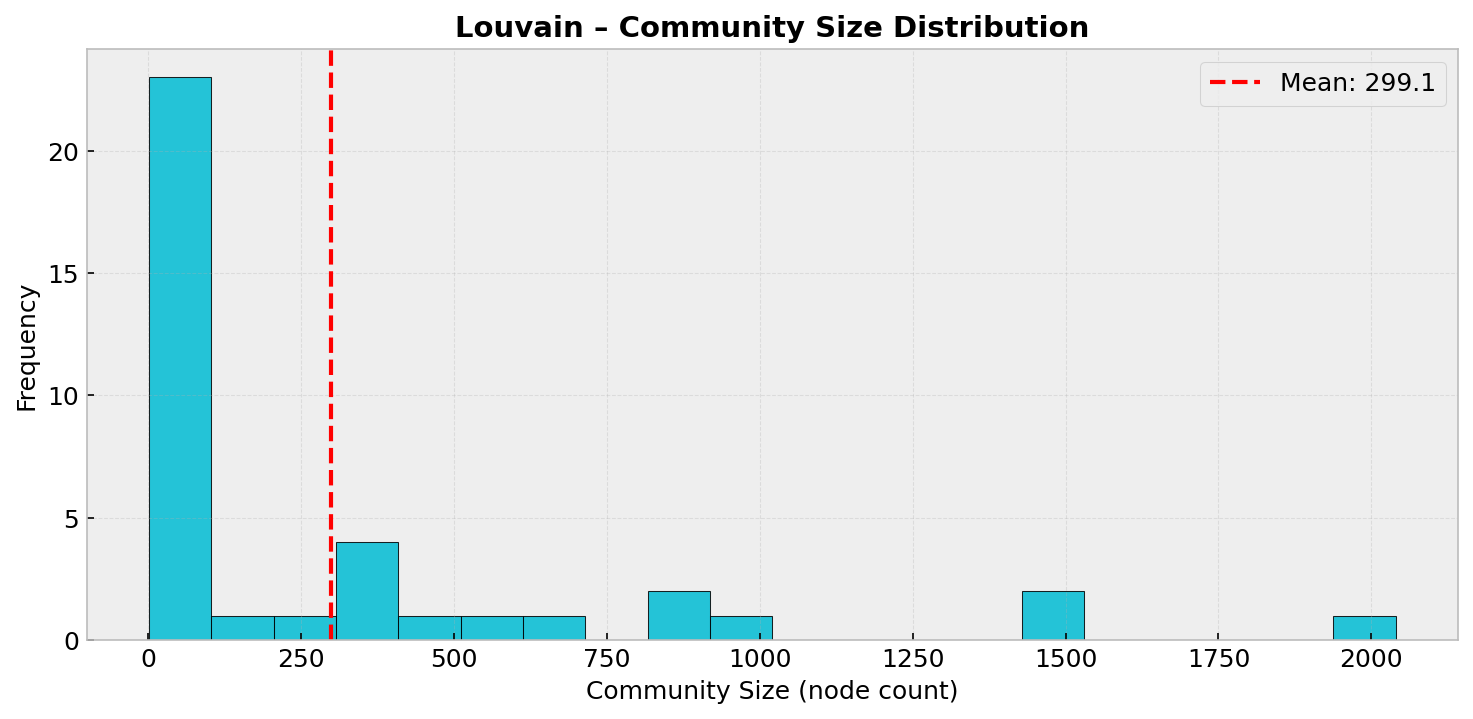
\includegraphics[width=0.75\textwidth]{figures/community-size-distribution-louvain.png}
    \caption{Distribution de taille des communautés Louvain (taille moyenne: 299.1 nœuds).}
    \label{fig:louvain-communities}
\end{figure}

\begin{figure}[H]
    \centering
    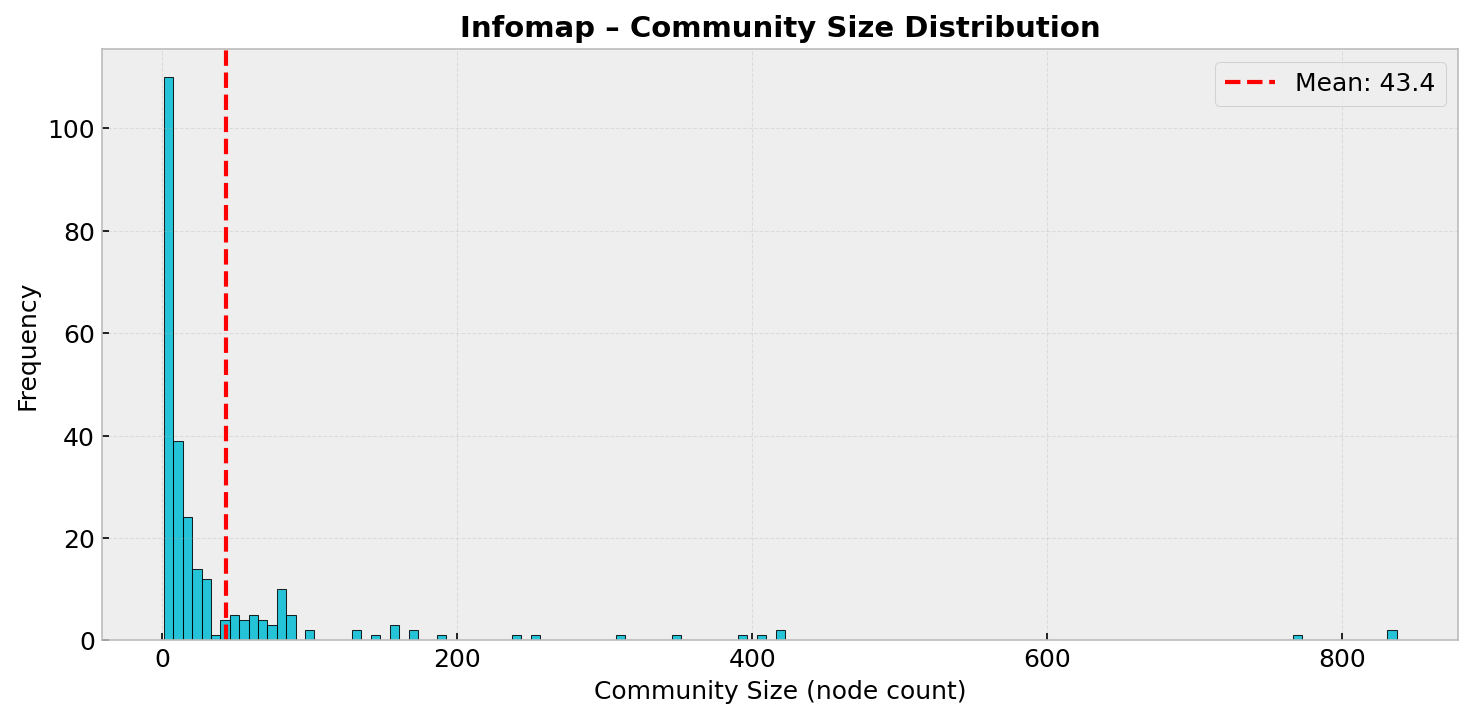
\includegraphics[width=0.75\textwidth]{figures/community-size-distribution-infomap.png}
    \caption{Distribution de taille des communautés Infomap (taille moyenne: 43.4 nœuds).}
    \label{fig:infomap-communities}
\end{figure}

\begin{table}[htbp]
\centering
\caption{Comparaison de détection de communautés: Louvain vs. Infomap.}
\label{tab:community-results}
\begin{tabular}{lrr}
\toprule
\textbf{Métrique} & \textbf{Louvain} & \textbf{Infomap} \\
\midrule
Modularité             & 0.6476 & 0.5998 \\
Nombre de communautés  & 38     & 262    \\
Taille max communauté  & 2\,040  & 837    \\
Taille moyenne communauté & 299.13 & 43.39  \\
Médiane communauté     & 3      & 11     \\
\bottomrule
\end{tabular}
\end{table}

Pour valider que les communautés détectées correspondent à des groupes sémantiquement cohérents, la Figure~\ref{fig:sim-dist} compare la similarité cosinus des arêtes intra-communauté contre les arêtes inter-communauté.

\begin{figure}[H]
    \centering
    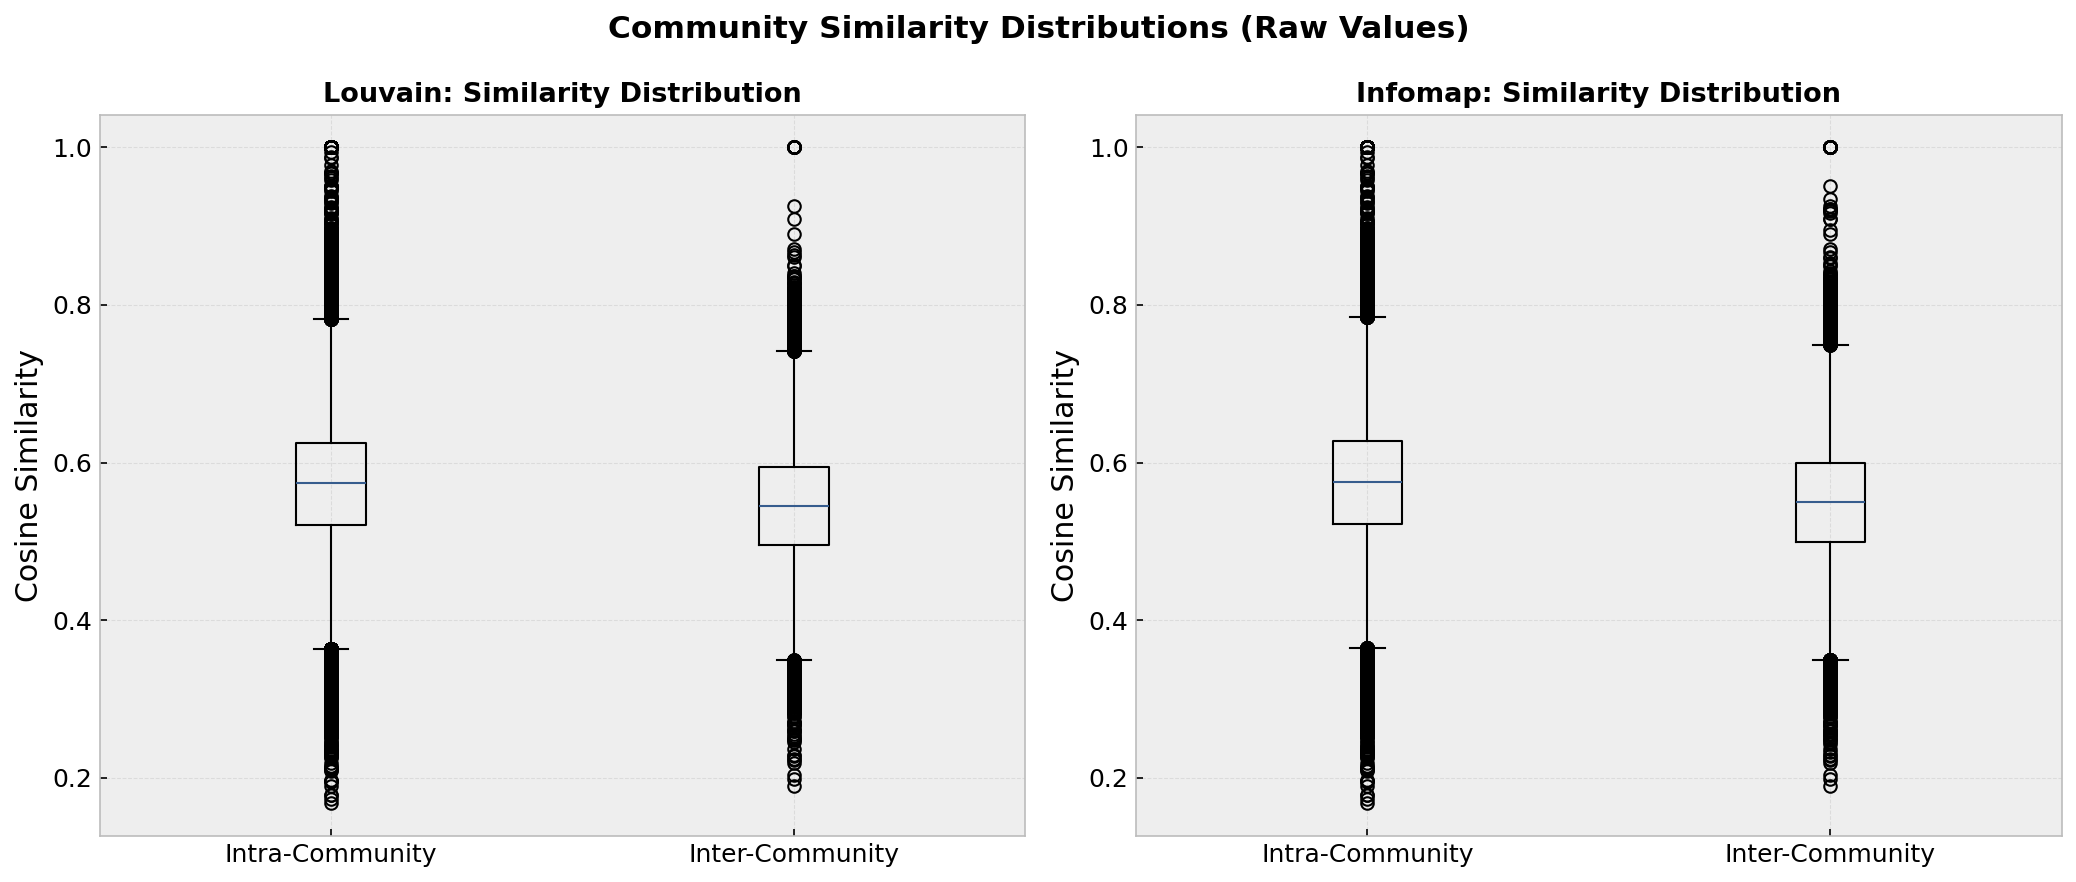
\includegraphics[width=0.75\textwidth]{figures/similarity-distributions.png}
    \caption{Similarité cosinus intra-communauté vs. inter-communauté: Louvain (gauche) et Infomap (droite).}
    \label{fig:sim-dist}
\end{figure}

\begin{table}[htbp]
\centering
\caption{Similarité cosinus moyenne: arêtes intra-communauté vs. inter-communauté.}
\label{tab:sim-community}
\begin{tabular}{lccc}
\toprule
\textbf{Algorithme} & \textbf{Intra-Communauté} & \textbf{Inter-Communauté} & \textbf{Différence} \\
\midrule
Louvain & 0.5729 & 0.5435 & $+0.0293$ \\
Infomap & 0.5748 & 0.5480 & $+0.0268$ \\
\bottomrule
\end{tabular}
\end{table}

Les deux algorithmes confirment que le graphe possède une structure de communautés significative. Louvain produit un petit nombre de grandes communautés (moyenne $\approx$299 nœuds), tandis qu'Infomap trouve plusieurs communautés plus petites et plus fines (moyenne $\approx$43 nœuds). Malgré la différence de granularité, les deux algorithmes s'accordent sur la conclusion clé (décrite dans le Tableau~\ref{tab:sim-community}): les nœuds au sein de la même communauté partagent constamment une similarité cosinus plus élevée que les nœuds de communautés différentes, validant le partitionnement structurel.

\subsection{Résultats de prédiction de liens GCN}

Les premières expériences GNN ont été conduites en utilisant un réseau convolutif sur graphes (GCN) comme base pour la tâche de prédiction de liens, telles que résumées dans le Tableau~\ref{tab:gcn-results}.

\begin{table}[htbp]
\centering
\caption{Dynamique d'entraînement GCN avec arrêt précoce.}
\label{tab:gcn-results}
\begin{tabular}{rrrr}
\toprule
\textbf{Époque} & \textbf{Loss} & \textbf{Val AUC} & \textbf{Notes} \\
\midrule
10 & 0.6356 & 0.8802 & \\
20 & 0.6059 & 0.8780 & \\
27 & --     & 0.8805 & Arrêt précoce (Meilleur Val AUC) \\
\midrule
\textbf{Test AUC (final)} & \multicolumn{3}{r}{\textbf{0.8653}} \\
\bottomrule
\end{tabular}
\end{table}

Le modèle GCN atteint rapidement une performance de validation forte dès l'époque 10. Avec l'arrêt précoce implémenté, le modèle arrête l'entraînement à l'époque 27, prévenant le surapprentissage sévère observé dans les exécutions prolongées de 100 époques. Cette base atteint un Test AUC final de 0.8653, démontrant que l'apprentissage topologique seul fournit un point de départ solide.

Le Test AUC final de \textbf{0.8653} établit une base solide pour la tâche de prédiction de liens.

\subsection{Résultats du système de recommandation}

Un système de recommandation basé sur le contenu combinant les embeddings BGE-M3 et Node2Vec basé sur SVD a été évalué sur 10 requêtes de sujets CS larges (Report-5), avec des exemples de résultats présentés dans le Tableau~\ref{tab:recommendation-results}.

\begin{table}[htbp]
\centering
\caption{Exemples de résultats de recommandation pour des requêtes de sujets larges.}
\label{tab:recommendation-results}
\begin{tabular}{lllr}
\toprule
\textbf{Requête} & \textbf{Recommandation Top-1} & \textbf{Similarité} & \textbf{Catégorie} \\
\midrule
Natural Language Processing & Machine Translation & 0.731 & NLP \\
Operating System & History of Operating Systems & 0.789 & Systems \\
Programming Language & Compiler & 0.769 & PL \\
Database & Database Design & 0.737 & Data \\
Cloud Computing & Cloud Storage & 0.772 & Distributed \\
World Wide Web & Line Mode Browser & 0.729 & Web \\
Adversarial Machine Learning & AlgoSec & 0.800 & Security* \\
Brownout (Software Eng.) & Belady's Anomaly & 0.823 & Systems* \\
Computer and Network Surveillance & Cyber Spying & 0.705 & Security \\
Quantum Programming & Cloud-based Quantum Computing & 0.726 & Quantum \\
\bottomrule
\end{tabular}
\end{table}

*Note: Certaines requêtes (Adversarial ML, Brownout) retournent des articles de clusters topics adjacents en raison du signal structurel de Node2Vec.

\subsection{Évaluation quantitative}

Le Tableau~\ref{tab:quantitative-eval} présente l'évaluation quantitative du système de recommandation sur les arêtes de test réservées.

\begin{table}[htbp]
\centering
\caption{Évaluation quantitative du système de recommandation.}
\label{tab:quantitative-eval}
\begin{tabular}{lr}
\toprule
\textbf{Métrique} & \textbf{Valeur} \\
\midrule
Arêtes de test évaluées & 63\,106 \\
Taux Hits@1 & 1.70\% (1\,075/63\,106) \\
Taux Hits@10 & 11.49\% (7\,249/63\,106) \\
MRR (Mean Reciprocal Rank) & 0.0548 \\
Ligne de base Hit@10 aléatoire & 0.086\% \\
Amélioration vs. aléatoire & $\approx$ 134$\times$ \\
\bottomrule
\end{tabular}
\end{table}

Le système combiné BGE-M3 + Node2Vec atteint un taux Hits@10 de 11.49\%, représentant une amélioration de \textbf{134$\times$} sur la recommandation aléatoire. Le MRR de 0.0548 indique que le voisin de test moyen apparaît au rang $\approx$18.

\section{Résumé et discussion}

Les résultats obtenus à ce jour démontrent la faisabilité de l'approche proposée:

\begin{itemize}
    \item Le graphe Custom-WikiCS présente une distribution des degrés en loi de puissance claire et une structure de communautés significative, confirmant que la structure d'hyperliens de Wikipédia encode les relations topiques
    \item Les paires d'articles liées sont significativement plus similaires (cosinus: 0.5726 vs. 0.4352 aléatoire), validant l'hypothèse que les hyperliens corrèlent avec la similarité sémantique
    \item La base GCN atteint Test AUC = 0.8653 avec arrêt précoce, établissant une base solide pour la prédiction de liens
    \item Le système de recommandation atteint 134$\times$ au-dessus de la ligne de base aléatoire, confirmant que les embeddings combinés captent à la fois les signaux sémantiques et structurels
\end{itemize}

Les domaines nécessitant une investigation plus approfondie incluent:
\begin{itemize}
    \item Implémentation du GAT et comparaison contre la base GCN
    \item Stratégies d'arrêt précoce et de régularisation
    \item Organisation hiérarchique du parcours par LLM (pas encore implémentée)
    \item Études d'ablation sur les stratégies de combinaison d'embeddings
\end{itemize}
